\chapter{Návrh experimentu}
\label{ch:design}

Experiment má odpovedať na dve otázky: ktorý útok zastaví ktorý prvok a koľko tento prvok stojí. Obe odpovede musia byť priraditeľné práve jednému prvku, preto platia dve pravidlá:

\begin{itemize}
  \item každá konfigurácia mení oproti svojej rodičovskej práve jeden ochranný prvok;
  \item vo všetkých konfiguráciách vrátane základnej beží ten istý CNI plugin (Cilium) s tými istými nastaveniami, takže rozdiel nemôže spôsobiť výmena sieťového riešenia.
\end{itemize}

\section{Testovacie prostredie}
\label{sec:testbed}

Cluster tvoria tri virtual machines na jednom hostiteľovi (MacBook Pro s Apple M4 Pro, 48~GB RAM): jeden riadiaci uzol a dva pracovné uzly, každý so 4~vCPU a 8~GiB RAM. Virtual machines spravuje Lima~\cite{lima} (Ubuntu 24.04 arm64, hypervízor vz) a spája ich spoločná sieť socket\_vmnet~\cite{socket-vmnet}, takže prevádzka medzi uzlami prechádza skutočným sieťovým rozhraním. Kubernetes zabezpečuje distribúcia k3s~\cite{k3s} bez vlastného CNI, bez vynucovania NetworkPolicy a bez kube-proxy; tieto úlohy preberá Cilium s náhradou kube-proxy a overlay sieťou VXLAN~\cite{cilium-docs,cilium-kpr}.

Testovanou aplikáciou je Bookinfo~\cite{istio-bookinfo} s verziami \texttt{reviews-v3} a \texttt{ratings-v2}, ktorá hodnotenia číta z MongoDB. Každý workload má vlastný ServiceAccount, aby mal v mesh vlastnú identitu. Pôvodne zvolená aplikácia Online Boutique~\cite{online-boutique} nevydáva image pre arm64, preto bola nahradená. Pody sú pripnuté na uzly tak, že každé volanie v grafe aplikácie prechádza medzi uzlami (obrázok~\ref{fig:testbed}). Verzie všetkých komponentov uvádza tabuľka~\ref{tab:versions}; celé prostredie vytvorí príkaz \texttt{make up}.

\begin{figure}[ht!]
  \centering
  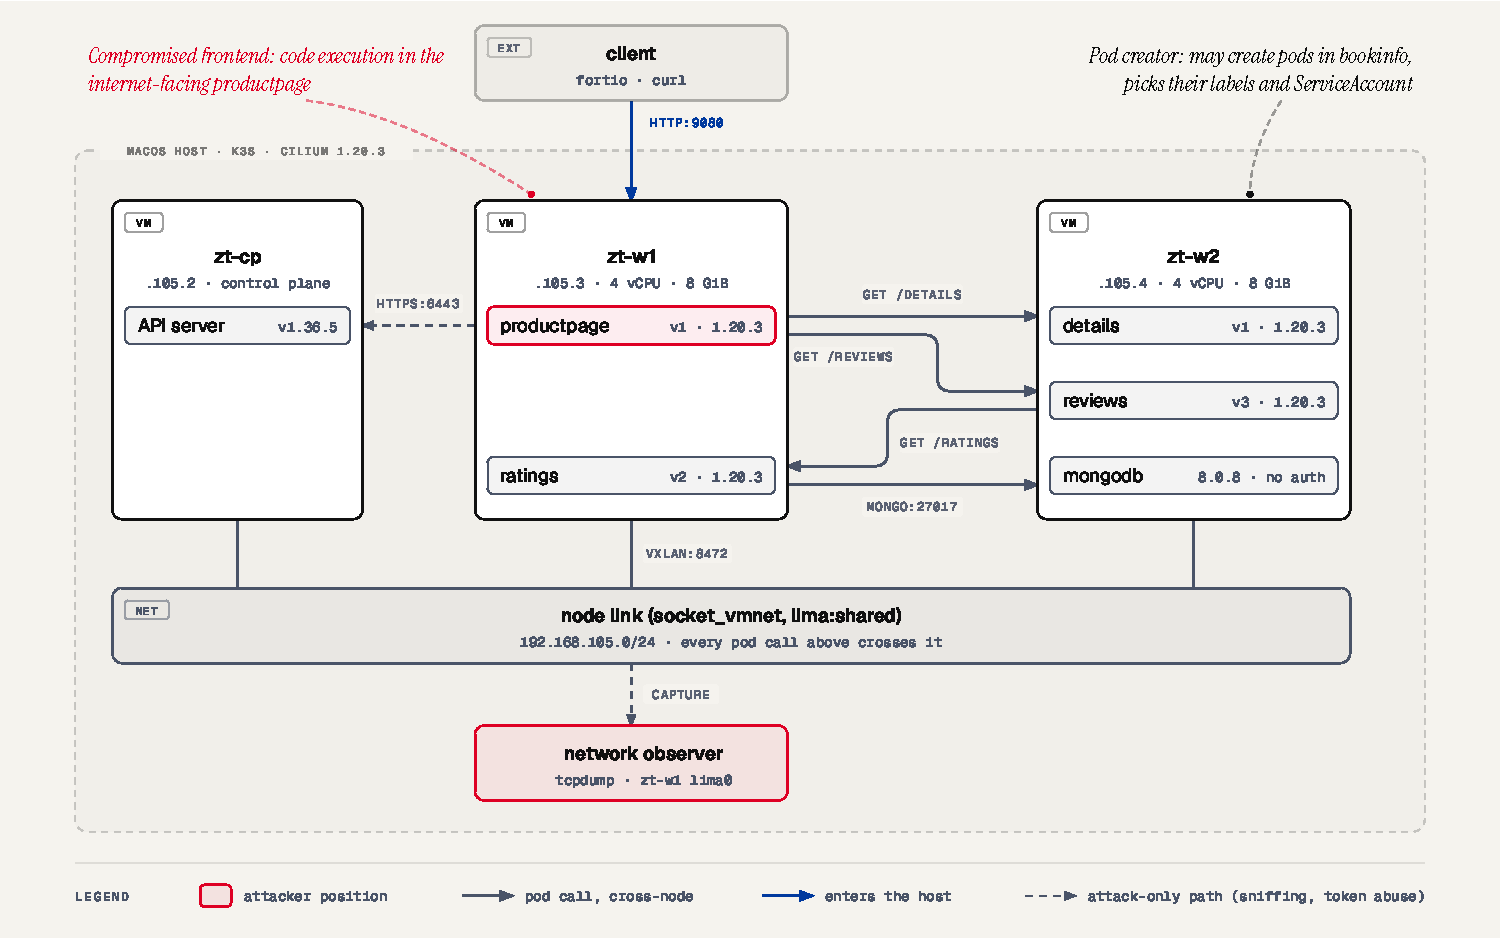
\includegraphics[width=\textwidth]{../figures/testbed.pdf}
  \caption{Testovacie prostredie: Bookinfo na troch virtual machines, každé volanie prechádza medzi uzlami; tri pozície útočníka.}
  \label{fig:testbed}
\end{figure}

\begin{table}[ht!]
  \centering
  \caption{Verzie komponentov}
  \label{tab:versions}
  \footnotesize
  \renewcommand{\arraystretch}{1.15}
  \begin{tabularx}{\textwidth}{@{}>{\raggedright\arraybackslash}p{3.4cm}>{\raggedright\arraybackslash}X@{}}
    \toprule
    Komponent & Verzia a nastavenie \\
    \midrule
    Lima, socket\_vmnet & 2.2.1, 1.2.2; sieť \texttt{lima:shared} (192.168.105.0/24) \\
    Kubernetes & k3s v1.36.5+k3s1 \\
    Cilium & 1.20.3; náhrada kube-proxy, VXLAN, nastavenia pre kompatibilitu s Istio vo všetkých konfiguráciách \\
    Šifrovanie medzi uzlami & Cilium WireGuard, modul jadra (Linux 6.8), iba prevádzka podov, MTU \texttt{cilium\_wg0} 1405 \\
    Service mesh & Istio 1.30.7 (Helm), režim sidecar, natívne sidecary \\
    Aplikácia & Bookinfo, image 1.20.3; MongoDB 8.0.8 \\
    Nástroje & Hubble 1.20.2, tshark 4.6.9, fortio 1.76.0, iperf3 3.22 \\
    \bottomrule
  \end{tabularx}
\end{table}

\section{Konfigurácie}
\label{sec:configurations}

Tabuľka~\ref{tab:configurations} uvádza konfigurácie a prvok, ktorý každá pridáva. Šifrovanie medzi uzlami a mesh mTLS sú súrodenci: obe vychádzajú zo segmentácie, aby sa dali priamo porovnať šifrovanie na úrovni uzla a na úrovni workloadu. Každú konfiguráciu nastaví jeden cieľ \texttt{make}, ktorý počká, kým aplikácia odpovedá po celej ceste.

\begin{table}[ht!]
  \centering
  \caption{Konfigurácie experimentu}
  \label{tab:configurations}
  \footnotesize
  \renewcommand{\arraystretch}{1.15}
  \begin{tabularx}{\textwidth}{@{}>{\raggedright\arraybackslash}p{3.2cm}>{\raggedright\arraybackslash}p{2.6cm}>{\raggedright\arraybackslash}X@{}}
    \toprule
    Konfigurácia & Rodič & Pridáva \\
    \midrule
    Základná & -- & Cilium bez politík a bez mesh \\
    Segmentácia & základná & default-deny NetworkPolicy s povolením iba grafu volaní a DNS; tokeny ServiceAccountov sa nepripájajú \\
    Šifrovanie medzi uzlami & segmentácia & transparentné šifrovanie Cilium WireGuard medzi uzlami \\
    Mesh mTLS & segmentácia & sidecary Istio, PeerAuthentication \texttt{STRICT} \\
    Autorizácia L7 & mesh mTLS & Istio AuthorizationPolicy pre \texttt{ratings} \\
    Mesh bez mTLS & segmentácia & sidecary Istio, mTLS vypnuté (\texttt{DISABLE}); iba na meranie réžie \\
    \bottomrule
  \end{tabularx}
\end{table}

Mesh mTLS pridáva naraz dva prvky: proxy v každom pode a mTLS. Pre bezpečnostné výsledky to nevadí, lebo útoky zastavuje mTLS. Pre meranie réžie sa však obe zložky oddelia konfiguráciou mesh bez mTLS, ktorá ponechá sidecary a vypne iba šifrovanie. Nastavenia Cilium potrebné pre spoluprácu s Istio sú súčasťou základnej konfigurácie, takže mesh mTLS mení len samotný mesh.

\section{Bezpečnostné testy}
\label{sec:attack-tests}

Každý útok z tabuľky~\ref{tab:attacks} má skript, ktorý ho vykoná proti aktuálnej konfigurácii; \texttt{make test} spustí všetky. Výsledok sa zapisuje do CSV spolu s očakávaným výsledkom a dôkaz sa ukladá do repozitára:

\begin{itemize}
  \item laterálny pohyb a podvrhnutie identity: výstup spojenia z podu útočníka a záznam zahodenia z Hubble, ktorý ukáže, že spojenie zastavila politika~\cite{hubble};
  \item odpočúvanie siete: záznam \texttt{tcpdump} na sieťovom rozhraní pracovného uzla počas legitímnej prevádzky, vyhodnotený nástrojom tshark~\cite{wireshark}; sleduje sa obsah aj metadáta (vnútorné adresy a porty podov); aktívna zmena prevádzky (T v STRIDE) sa netestuje;
  \item neoprávnená operácia a kompromitovaná služba: požiadavky z ephemeral containera v pode \texttt{reviews}~\cite{k8s-ephemeral-containers};
  \item zneužitie tokenu: štyri kontroly z tabuľky~\ref{tab:token}.
\end{itemize}

Most siete na hostiteľovi nevidí rámce medzi virtual machines, preto sa prevádzka zaznamenáva priamo na rozhraní uzla vo virtual machine. Pri neoprávnenej operácii \texttt{ratings-v2} odpovedá na zápis chybou 501, lebo zápis implementuje iba verzia v1. Verdikt preto nezávisí od zmeny dát, ale od toho, či požiadavka dorazí do aplikácie (akákoľvek odpoveď \texttt{ratings}), alebo ju odmietne sidecar (403).

Tabuľka~\ref{tab:expected} uvádza očakávané výsledky, teda hypotézy, ktoré testy overujú. Namerané výsledky sú v kapitole~\ref{ch:security-results}.

\begin{table}[ht!]
  \centering
  \caption{Očakávané výsledky útokov (\enquote{prejde} alebo \enquote{zastavený})}
  \label{tab:expected}
  \footnotesize
  \renewcommand{\arraystretch}{1.15}
  \begin{tabularx}{\textwidth}{@{}>{\raggedright\arraybackslash}X>{\centering\arraybackslash}p{1.65cm}>{\centering\arraybackslash}p{1.65cm}>{\centering\arraybackslash}p{1.65cm}>{\centering\arraybackslash}p{1.65cm}>{\centering\arraybackslash}p{1.65cm}@{}}
    \toprule
    Útok & Základná & Segmen\-tácia & Šifrovanie medzi uzlami & Mesh mTLS & Autori\-zácia L7 \\
    \midrule
    Laterálny pohyb & prejde & zastavený & zastavený & zastavený & zastavený \\
    Odpočúvanie siete & prejde & prejde & zastavený & zastavený & zastavený \\
    Podvrhnutie, mimo mesh & prejde & prejde & prejde & zastavený & zastavený \\
    Podvrhnutie, iný SA & prejde & prejde & prejde & prejde & zastavený \\
    Podvrhnutie, ukradnutý SA & prejde & prejde & prejde & prejde & prejde \\
    Neoprávnená operácia & prejde & prejde & prejde & prejde & zastavený \\
    Kompromitovaná služba & prejde & prejde & prejde & prejde & prejde \\
    Zneužitie tokenu & prejde & zastavený & zastavený & zastavený & zastavený \\
    \bottomrule
  \end{tabularx}
\end{table}

\section{Meranie réžie}
\label{sec:measurement-design}

Réžia sa meria ako rozdiel medzi konfiguráciou a jej rodičom, takže každý rozdiel zodpovedá jednému prvku (tabuľka~\ref{tab:deltas}).

\begin{table}[ht!]
  \centering
  \caption{Porovnávané dvojice konfigurácií}
  \label{tab:deltas}
  \footnotesize
  \renewcommand{\arraystretch}{1.15}
  \begin{tabularx}{\textwidth}{@{}>{\raggedright\arraybackslash}p{6.2cm}>{\raggedright\arraybackslash}X@{}}
    \toprule
    Porovnanie & Meraný prvok \\
    \midrule
    Segmentácia oproti základnej & vynucovanie NetworkPolicy v eBPF \\
    Šifrovanie medzi uzlami oproti segmentácii & WireGuard medzi uzlami \\
    Mesh bez mTLS oproti segmentácii & sidecar proxy bez šifrovania \\
    Mesh mTLS oproti mesh bez mTLS & mTLS v proxy \\
    Mesh mTLS oproti šifrovaniu medzi uzlami & šifrovanie na úrovni workloadu oproti úrovni uzla \\
    Autorizácia L7 oproti mesh mTLS & vyhodnotenie autorizačnej politiky v proxy \\
    \bottomrule
  \end{tabularx}
\end{table}

Merajú sa tri veličiny:

\begin{itemize}
  \item latencia (p50, p95, p99) nástrojom fortio pri konštantnej záťaži v požiadavkách za sekundu~\cite{fortio}, na troch cestách: medzi podmi fortio na tom istom uzle, medzi podmi na rôznych uzloch a cez celú aplikáciu od \texttt{productpage};
  \item priepustnosť TCP jedného toku nástrojom iperf3~\cite{iperf3} na tom istom uzle a medzi uzlami; raz aj medzi uzlami bez podov a CNI ako strop linky medzi virtual machines;
  \item spotreba CPU a pamäte uzlov, agentov Cilium, sidecarov a podov aplikácie (\texttt{kubectl top}) počas meraní latencie.
\end{itemize}

Odvodenou metrikou je spotreba CPU na jednotku práce (milijadrá na 1000 požiadaviek, resp. na Gbit/s), ktorá je na notebooku stabilnejšia než absolútna latencia alebo priepustnosť.

Postup merania:

\begin{enumerate}
  \item Kalibrácia: zistí sa saturačná záťaž cesty cez celú aplikáciu v najnáročnejšej konfigurácii (autorizácia L7) a pre všetky konfigurácie sa použije približne jej polovica, aby sa žiadna nemerala v saturácii.
  \item Pre každú konfiguráciu a cestu jeden zahrievací beh, ktorý sa zahodí, a potom päť behov (fortio 60~s, iperf3 30~s bez prvých 5~s).
  \item Konfigurácie sa striedajú po kolách, aby pomalý drift prostredia nedopadol na jednu z nich.
  \item Výsledkom je medián z behov a rozsah od minima po maximum.
\end{enumerate}

Veľkosť virtual machines, verzie a rozmiestnenie podov sú vo všetkých konfiguráciách rovnaké; počas merania nebeží na hostiteľovi iná záťaž. Všetky virtual machines bežia na jednom notebooku a prevádzka medzi uzlami ho neopúšťa, preto majú význam iba relatívne rozdiely medzi konfiguráciami, nie absolútne hodnoty.
